\documentclass[lettersize,journal]{IEEEtran}
\usepackage{amsmath,amsfonts}
\usepackage{algorithmic}
\usepackage{algorithm}
\usepackage{array}
\usepackage[caption=false,font=normalsize,labelfont=sf,textfont=sf]{subfig}
\usepackage{textcomp}
\usepackage{stfloats}
\usepackage{url}
\usepackage{verbatim}
\usepackage{graphicx}
\usepackage{cite}
\hyphenation{op-tical net-works semi-conduc-tor IEEE-Xplore}
% updated with editorial comments 8/9/2021

\begin{document}

\title{A Sample Article Using IEEEtran.cls\\ for IEEE Journals and Transactions}

\author{IEEE Publication Technology,~\IEEEmembership{Staff,~IEEE,}
        % <-this % stops a space
\thanks{This paper was produced by the IEEE Publication Technology Group. They are in Piscataway, NJ.}% <-this % stops a space
\thanks{Manuscript received April 19, 2021; revised August 16, 2021.}}

% The paper headers
\markboth{Journal of \LaTeX\ Class Files,~Vol.~14, No.~8, August~2021}%
{Shell \MakeLowercase{\textit{et al.}}: A Sample Article Using IEEEtran.cls for IEEE Journals}

\IEEEpubid{0000--0000/00\$00.00~\copyright~2021 IEEE}
% Remember, if you use this you must call \IEEEpubidadjcol in the second
% column for its text to clear the IEEEpubid mark.

\maketitle

\begin{abstract}
This document describes the most common article elements and how to use the IEEEtran class with \LaTeX \ to produce files that are suitable for submission to the IEEE.  IEEEtran can produce conference, journal, and technical note (correspondence) papers with a suitable choice of class options. 
\end{abstract}

\begin{IEEEkeywords}
Article submission, IEEE, IEEEtran, journal, \LaTeX, paper, template, typesetting.
\end{IEEEkeywords}

\section{Introduction}
\IEEEPARstart{A}{s} per studies, one-third of music streaming on smartphones is intended to influence affective states \cite{wadley2019use}. According to a recent survey, 73.8\% of respondents reported using online music as a means of managing their emotions \cite{martin2021music}. Using social media applications was the most effective technique to self-regulate mood during the COVID-19 pandemic. Pre-pandemic, a different survey found that 87\% of teens and adults would go online for ways to deal with stress, anxiety, or depression, but just 20\% of them would consider seeking professional help \cite{rideout2018digital}. Some instances of emotions driving smartphone usage in daily life include listening to music while exercising, watching online videos during daily commutes, scrolling through social media while waiting in a queue, and browsing shopping websites at the workplace.


The practice of consciously modifying one's affective state is called emotion regulation (ER). The ability to successfully perform emotion regulation is essential to function effectively in everyday life, to act appropriately in everyday interactions, or merely for hedonic purposes. The ubiquity of digital technology has produced a plethora of prospects for understanding, managing and influencing the world we live in. Today, digital technology is being used as a tool to strategically influence our affective states (such as emotions, mood and stress levels), a process known as digital emotion regulation (DER). In addition to its novelty and scope, understanding digital emotion regulation can facilitate the advancement of the ethical design, development, and application of technology.


The rise in popularity of social media applications has led to significant virtualisation of engagement activities in our lives. Since these applications provide a variety of dimensions for expression and consumption, traditional forms of leisure and amusement have also been revolutionised by this digitisation. The COVID-19 pandemic made it difficult to socialise offline, thus more people than ever are choosing to spend their social lives online. Emotions are intertwined in our daily affairs and shape our interactions because they are an integral part of human behaviour and influence how we think and act. Our experiences elicit emotional responses, and these emotions frame our actions. The same is also true for digital technology and social media. It has been observed that emotional states impact interactions with technology, such as joystick movements, typing errors, as well as typing speed. Recent studies have established a correlation between emotional states and the number of application launches, duration of application use, and type of application used, demonstrating that the relationship between emotions and social media use is bidirectional \cite{sarsenbayeva2020does}. People have created a toolkit that allows them to actively appropriate and integrate a variety of applications to manage emotions in everyday life \cite{smith2022digital}. Scrolling through social media feeds for distraction, watching cat videos for stress relief, texting a friend to seek support, following an inspirational person to focus on success, and sharing emotions through status updates are a few examples of emotion regulation via social media platforms. The omnipresence of social media applications has optimised our ability to regulate emotions at any time or place by allowing us to fine-tune our strategies for specific situations and engage in emotion regulation more frequently.

Understanding emotion regulation necessitates learning about the process of emotion regulation as well as the motivation for doing so. Gross's process model describes how people regulate their emotions by classifying the strategies for emotion regulation into five categories based on when they are encountered in the sequence of emotion generation \cite{wadley2020digital}. Situation selection is the first intervention, which entails going into situations that might evoke desired emotions or staying away from scenarios that might induce undesirable emotions. Situation modification makes it possible to control emotions by directly altering specific aspects of a situation after it has been encountered, however before an emotional reaction has fully formed. This is accomplished by using attentional deployment to shift one's focus from or toward emotion-relevant features, or by reevaluating a situation to change the way its emotional impact through cognitive change. Lastly, response modulation can be used to change the physiological, behavioural, or experiential components of an emotional response even after it has already occurred. For instance, by exhibiting intensified facial expressions. Tamir's motive taxonomy, which divides the goal of emotion regulation into two categories, hedonic and instrumental, with additional classifications, may be used to explain emotion regulation motivations. Hedonic motives (Prohedonic and Contrahedonic) entail engaging in emotion regulation in order to experience or avoid certain emotions; typically, pleasant emotions are enhanced while painful emotions are diminished. Instrumental motives (Performance, Epistemic, and Social) are motivations that people have when they believe that certain affective states will help them achieve a goal, meet performance objectives, or demonstrate socially acceptable expressions and behaviours \cite{wadley2020digital}.

The examples discussed thus far in this article are cases of intrinsic ER, in which people intend to alter their own affective states; however, in digital technologies, extrinsic ER is an essential component, where people intentionally try to influence the emotional state of others. Social media platforms allow users to create identifiable profiles, represent public connections and consume, produce, and/or interact with a wide range of user-generated content created by their connections on the site. These applications consistently harbour communication among millions of people from all over the world and hence contain traces of emotional expression in abundance. Since the virtual world offers an opportunity to network with people beyond geographical boundaries, exposure to the expressions of others amplifies, which has the potential to influence the emotions, actions and online behaviours of the users. Because user engagement is a key factor in the success of social media platforms, and exposure to emotion increases it, social media companies have strategically used the emotional effects of activities on social media platforms to improve user experience and fuel user participation. This intervention by digital media companies to boost the intensity and frequency of expression has resulted in a rise in online emotion contagion, which is the spontaneous spread and convergence of emotion based on exposure \cite{goldenberg2020digital}. According to ER psychological research, emotion contagion can be caused by extrinsic emotion regulation \cite{elfenbein2014many}. Online movements such as \#MeToo and toilet paper hoarding during COVID-19, which rely on users' connected behaviours and have an impact on users' offline lives as well, emerged as a result of emotional contagion. Implicit emotion regulation, which does not involve a conscious desire to alter emotional responses, may also play a role in the development of connective action. Nonetheless, through the disproportionate induction and convergence of emotion, it generates social dysfunction and online toxicity.


There is still a substantial difference in social behaviour between online and offline, even though as technology becomes a more accepted part of our life, the boundary between the real and the virtual is dissolving. Although online toxicity has been well understood, recognised, and intensively studied for a few years now, combatting measures are challenging to implement due to the nature of online media environments, where the context of user behaviours cannot always be extracted. Anonymity in social media platforms keeps the users behind the safety of a keyboard. This lack of accountability in social media platforms has resulted in poverty in online well-being. What is acceptable online (due to lack of mediation, moderation, or other restrictions), may not be accepted offline. This emphasises the importance of researching how emotion regulation could be utilized to ensure consistent well-being online by enabling ethical design and development in social media applications. As a result, this work sheds light on recent advances in DER for social media applications. It focuses on the applications of identifying and understanding emotion regulation on these platforms by providing a comparative analysis of emotion regulation strategies used by users on various social media applications. Therefore, the following are the main contributions of this work:
\begin{itemize}
    \item We provide an overview of digital emotion regulation in social media applications, as well as a synthesis of recent research on emotion regulation interventions for social media.
    \item We share our findings from analysing a variety of literature articles on how different social media applications are used at various stages of the emotion regulation process.
    \item We offer a theoretical analysis of the extrinsic emotion regulation strategies prevalent on social media platforms which may help improve online well-being.
\end{itemize}

The rest of this article is structured as follows. We begin by discussing the evolution of digital emotion regulation in social media platforms, followed by a description of the popular approaches used to analyse emotions in social media platforms (the 'how' and 'what'). Then we present some applications of understanding emotional regulation in social media applications, as well as methods for implementing them. Subsequently, we present a comparative analysis of emotion regulation strategies employed by users on various social media applications. Finally, we identify gaps in the literature and conclude the article with some future directions.


\section{Emotion Regulation in Social Media}
HCI research has seen an increase in interest in the design and development of technological interventions that can help and support emotion regulation. This renewed interest originates from the realisation and recognition that effective emotion regulation is a vital aspect of mental health. Over the last decade, there has been a lot of research into technology-enabled mental health support and the development of a diverse array of tools designed to assist with emotion regulation. The availability and popularity of low-cost wearable sensors and extensively configurable bio-feedback devices fueled this. Another factor that has contributed to this advancement is psychological research in the field of emotion regulation, which now recognises effective ER as a key factor in personal well-being and is using it as a trans-diagnostic intervention for mental health disorders. This section summarises the recent elements of research and development that have emerged in the field of digital emotion regulation. 

\subsection{Observational Studies}
Recent studies have examined how people combine a variety of social media applications, such as video streaming platforms, discussion forums, online games, and music, to regulate their emotions, thoughts, and behaviours. A common technique known as "mental reset" has been observed, in which individuals employ social media apps to distract themselves from overwhelming emotions. Several diary studies have been conducted to better understand various aspects of everyday emotion regulation in isolation, such as the use of social media to avert homesickness and university students' use of music streaming platforms. Individuals' multitasking and passive scrolling habits on social media apps have also been explored in studies revealing how people voluntarily take breaks from social media to mitigate negativity or uphold a sense of equilibrium, as well as highlighting the practice of interpersonal emotion regulation in discussion forums \cite{smith2022digital}. It was discovered that active social media usage had a higher rate of emotion regulation than passive usage, which provided superior support for rest and recovery \cite{hossain2022motivational}. The effect of the pandemic on young people's digital emotion regulation habits has also been studied, and it indicates that while the lockdown made people's emotion regulation practises more uniform, it also increased their reliance on technology and increased their proclivity to use emotion suppression strategies \cite{tag2022impact}. Computing research in digital emotion regulation draws on psychological research literature by employing Gross's process model for classifying ER strategies and practices, as well as Tamir's motives for identifying the goals of performing ER. Altogether, these studies show the variety of digital technologies people use to regulate their emotions in their daily lives. They emphasise the importance of the technologies packed into these devices and the need to boost well-being online, in addition to the growing significance of digital technologies in promoting mental well-being on a global scale.
\subsection{Design and Evaluation of Novel Tools}
This body of research involves the development of interventions that seek to support, develop, or guide emotion regulation skills or help individuals use such skills in challenging situations. The process of emotion regulation occurs in four stages: identifying the need to regulate emotions, selecting an appropriate strategy, implementing it, and then monitoring the regulated state to determine whether additional regulation is required. Technology-enabled interventions have aimed at either supporting a specific ER strategy or boosting emotional awareness during the identification or monitoring stages \cite{slovak2022designing}. They include experience-based design components which primarily focus on bio-feedback or implicit target responses to nudge users subconsciously toward specific physiological states via haptic interaction, such as guided slow breathing for car drivers \cite{smith2022digital}. These involve features for both on-the-spot and offline support. On-the-spot support systems use triggers to guide or support users' during the emotion regulation processes, and they can provide either one-time reminders or ongoing haptic support. Offline support mechanisms use interactivity to generate a personalised emotion regulation cycle, such as visualising a timeline of emotional patterns to structure users' reflections. Recent advancements have also seen didactic intervention components that rely on reminder-based recommender systems, such as suggesting specific ER strategies to users and facilitating emotion awareness by prompting users to consider how they feel or felt. These works investigate new design possibilities for DER, and by examining how these designs affect users, they open up new avenues for research in this field.

\section{Where to Get \LaTeX \ Help --- User Groups}
The following online groups are helpful to beginning and experienced \LaTeX\ users. A search through their archives can provide many answers to common questions.
\begin{list}{}{}
\item{\url{http://www.latex-community.org/}} 
\item{\url{https://tex.stackexchange.com/} }
\end{list}

\section{Other Resources}
See \cite{ref1,ref2,ref3,ref4,ref5} for resources on formatting math into text and additional help in working with \LaTeX .

\section{Text}
For some of the remainer of this sample we will use dummy text to fill out paragraphs rather than use live text that may violate a copyright.

Itam, que ipiti sum dem velit la sum et dionet quatibus apitet voloritet audam, qui aliciant voloreicid quaspe volorem ut maximusandit faccum conemporerum aut ellatur, nobis arcimus.
Fugit odi ut pliquia incitium latum que cusapere perit molupta eaquaeria quod ut optatem poreiur? Quiaerr ovitior suntiant litio bearciur?

Onseque sequaes rectur autate minullore nusae nestiberum, sum voluptatio. Et ratem sequiam quaspername nos rem repudandae volum consequis nos eium aut as molupta tectum ulparumquam ut maximillesti consequas quas inctia cum volectinusa porrum unt eius cusaest exeritatur? Nias es enist fugit pa vollum reium essusam nist et pa aceaqui quo elibusdandis deligendus que nullaci lloreri bla que sa coreriam explacc atiumquos simolorpore, non prehendunt lam que occum\cite{ref6} si aut aut maximus eliaeruntia dia sequiamenime natem sendae ipidemp orehend uciisi omnienetus most verum, ommolendi omnimus, est, veni aut ipsa volendelist mo conserum volores estisciis recessi nveles ut poressitatur sitiis ex endi diti volum dolupta aut aut odi as eatquo cullabo remquis toreptum et des accus dolende pores sequas dolores tinust quas expel moditae ne sum quiatis nis endipie nihilis etum fugiae audi dia quiasit quibus.
\IEEEpubidadjcol
Ibus el et quatemo luptatque doluptaest et pe volent rem ipidusa eribus utem venimolorae dera qui acea quam etur aceruptat.
Gias anis doluptaspic tem et aliquis alique inctiuntiur?

Sedigent, si aligend elibuscid ut et ium volo tem eictore pellore ritatus ut ut ullatus in con con pere nos ab ium di tem aliqui od magnit repta volectur suntio. Nam isquiante doluptis essit, ut eos suntionsecto debitiur sum ea ipitiis adipit, oditiore, a dolorerempos aut harum ius, atquat.

Rum rem ditinti sciendunti volupiciendi sequiae nonsect oreniatur, volores sition ressimil inus solut ea volum harumqui to see\eqref{deqn_ex1a} mint aut quat eos explis ad quodi debis deliqui aspel earcius.

\begin{equation}
\label{deqn_ex1a}
x = \sum_{i=0}^{n} 2{i} Q.
\end{equation}

Alis nime volorempera perferi sitio denim repudae pre ducilit atatet volecte ssimillorae dolore, ut pel ipsa nonsequiam in re nus maiost et que dolor sunt eturita tibusanis eatent a aut et dio blaudit reptibu scipitem liquia consequodi od unto ipsae. Et enitia vel et experferum quiat harum sa net faccae dolut voloria nem. Bus ut labo. Ita eum repraer rovitia samendit aut et volupta tecupti busant omni quiae porro que nossimodic temquis anto blacita conse nis am, que ereperum eumquam quaescil imenisci quae magnimos recus ilibeaque cum etum iliate prae parumquatemo blaceaquiam quundia dit apienditem rerit re eici quaes eos sinvers pelecabo. Namendignis as exerupit aut magnim ium illabor roratecte plic tem res apiscipsam et vernat untur a deliquaest que non cus eat ea dolupiducim fugiam volum hil ius dolo eaquis sitis aut landesto quo corerest et auditaquas ditae voloribus, qui optaspis exero cusa am, ut plibus.


\section{Some Common Elements}
\subsection{Sections and Subsections}
Enumeration of section headings is desirable, but not required. When numbered, please be consistent throughout the article, that is, all headings and all levels of section headings in the article should be enumerated. Primary headings are designated with Roman numerals, secondary with capital letters, tertiary with Arabic numbers; and quaternary with lowercase letters. Reference and Acknowledgment headings are unlike all other section headings in text. They are never enumerated. They are simply primary headings without labels, regardless of whether the other headings in the article are enumerated. 

\subsection{Citations to the Bibliography}
The coding for the citations is made with the \LaTeX\ $\backslash${\tt{cite}} command. 
This will display as: see \cite{ref1}.

For multiple citations code as follows: {\tt{$\backslash$cite\{ref1,ref2,ref3\}}}
 which will produce \cite{ref1,ref2,ref3}. For reference ranges that are not consecutive code as {\tt{$\backslash$cite\{ref1,ref2,ref3,ref9\}}} which will produce  \cite{ref1,ref2,ref3,ref9}

\subsection{Lists}
In this section, we will consider three types of lists: simple unnumbered, numbered, and bulleted. There have been many options added to IEEEtran to enhance the creation of lists. If your lists are more complex than those shown below, please refer to the original ``IEEEtran\_HOWTO.pdf'' for additional options.\\

\subsubsection*{\bf A plain  unnumbered list}
\begin{list}{}{}
\item{bare\_jrnl.tex}
\item{bare\_conf.tex}
\item{bare\_jrnl\_compsoc.tex}
\item{bare\_conf\_compsoc.tex}
\item{bare\_jrnl\_comsoc.tex}
\end{list}

\subsubsection*{\bf A simple numbered list}
\begin{enumerate}
\item{bare\_jrnl.tex}
\item{bare\_conf.tex}
\item{bare\_jrnl\_compsoc.tex}
\item{bare\_conf\_compsoc.tex}
\item{bare\_jrnl\_comsoc.tex}
\end{enumerate}

\subsubsection*{\bf A simple bulleted list}
\begin{itemize}
\item{bare\_jrnl.tex}
\item{bare\_conf.tex}
\item{bare\_jrnl\_compsoc.tex}
\item{bare\_conf\_compsoc.tex}
\item{bare\_jrnl\_comsoc.tex}
\end{itemize}





\subsection{Figures}
Fig. 1 is an example of a floating figure using the graphicx package.
 Note that $\backslash${\tt{label}} must occur AFTER (or within) $\backslash${\tt{caption}}.
 For figures, $\backslash${\tt{caption}} should occur after the $\backslash${\tt{includegraphics}}.

\begin{figure}[!t]
\centering
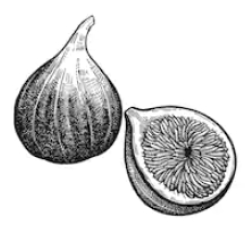
\includegraphics[width=2.5in]{fig1}
\caption{Simulation results for the network.}
\label{fig_1}
\end{figure}

Fig. 2(a) and 2(b) is an example of a double column floating figure using two subfigures.
 (The subfig.sty package must be loaded for this to work.)
 The subfigure $\backslash${\tt{label}} commands are set within each subfloat command,
 and the $\backslash${\tt{label}} for the overall figure must come after $\backslash${\tt{caption}}.
 $\backslash${\tt{hfil}} is used as a separator to get equal spacing.
 The combined width of all the parts of the figure should do not exceed the text width or a line break will occur.
%
\begin{figure*}[!t]
\centering
\subfloat[]{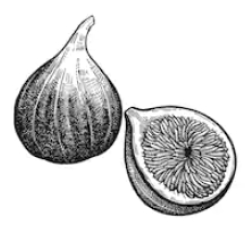
\includegraphics[width=2.5in]{fig1}%
\label{fig_first_case}}
\hfil
\subfloat[]{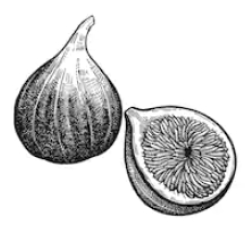
\includegraphics[width=2.5in]{fig1}%
\label{fig_second_case}}
\caption{Dae. Ad quatur autat ut porepel itemoles dolor autem fuga. Bus quia con nessunti as remo di quatus non perum que nimus. (a) Case I. (b) Case II.}
\label{fig_sim}
\end{figure*}

Note that often IEEE papers with multi-part figures do not place the labels within the image itself (using the optional argument to $\backslash${\tt{subfloat}}[]), but instead will
 reference/describe all of them (a), (b), etc., within the main caption.
 Be aware that for subfig.sty to generate the (a), (b), etc., subfigure
 labels, the optional argument to $\backslash${\tt{subfloat}} must be present. If a
 subcaption is not desired, leave its contents blank,
 e.g.,$\backslash${\tt{subfloat}}[].


 

\section{Tables}
Note that, for IEEE-style tables, the
 $\backslash${\tt{caption}} command should come BEFORE the table. Table captions use title case. Articles (a, an, the), coordinating conjunctions (and, but, for, or, nor), and most short prepositions are lowercase unless they are the first or last word. Table text will default to $\backslash${\tt{footnotesize}} as
 the IEEE normally uses this smaller font for tables.
 The $\backslash${\tt{label}} must come after $\backslash${\tt{caption}} as always.
 
\begin{table}[!t]
\caption{An Example of a Table\label{tab:table1}}
\centering
\begin{tabular}{|c||c|}
\hline
One & Two\\
\hline
Three & Four\\
\hline
\end{tabular}
\end{table}

\section{Algorithms}
Algorithms should be numbered and include a short title. They are set off from the text with rules above and below the title and after the last line.

\begin{algorithm}[H]
\caption{Weighted Tanimoto ELM.}\label{alg:alg1}
\begin{algorithmic}
\STATE 
\STATE {\textsc{TRAIN}}$(\mathbf{X} \mathbf{T})$
\STATE \hspace{0.5cm}$ \textbf{select randomly } W \subset \mathbf{X}  $
\STATE \hspace{0.5cm}$ N_\mathbf{t} \gets | \{ i : \mathbf{t}_i = \mathbf{t} \} | $ \textbf{ for } $ \mathbf{t}= -1,+1 $
\STATE \hspace{0.5cm}$ B_i \gets \sqrt{ \textsc{max}(N_{-1},N_{+1}) / N_{\mathbf{t}_i} } $ \textbf{ for } $ i = 1,...,N $
\STATE \hspace{0.5cm}$ \hat{\mathbf{H}} \gets  B \cdot (\mathbf{X}^T\textbf{W})/( \mathbb{1}\mathbf{X} + \mathbb{1}\textbf{W} - \mathbf{X}^T\textbf{W} ) $
\STATE \hspace{0.5cm}$ \beta \gets \left ( I/C + \hat{\mathbf{H}}^T\hat{\mathbf{H}} \right )^{-1}(\hat{\mathbf{H}}^T B\cdot \mathbf{T})  $
\STATE \hspace{0.5cm}\textbf{return}  $\textbf{W},  \beta $
\STATE 
\STATE {\textsc{PREDICT}}$(\mathbf{X} )$
\STATE \hspace{0.5cm}$ \mathbf{H} \gets  (\mathbf{X}^T\textbf{W} )/( \mathbb{1}\mathbf{X}  + \mathbb{1}\textbf{W}- \mathbf{X}^T\textbf{W}  ) $
\STATE \hspace{0.5cm}\textbf{return}  $\textsc{sign}( \mathbf{H} \beta )$
\end{algorithmic}
\label{alg1}
\end{algorithm}

Que sunt eum lam eos si dic to estist, culluptium quid qui nestrum nobis reiumquiatur minimus minctem. Ro moluptat fuga. Itatquiam ut laborpo rersped exceres vollandi repudaerem. Ulparci sunt, qui doluptaquis sumquia ndestiu sapient iorepella sunti veribus. Ro moluptat fuga. Itatquiam ut laborpo rersped exceres vollandi repudaerem. 
\section{Mathematical Typography \\ and Why It Matters}

Typographical conventions for mathematical formulas have been developed to {\bf provide uniformity and clarity of presentation across mathematical texts}. This enables the readers of those texts to both understand the author's ideas and to grasp new concepts quickly. While software such as \LaTeX \ and MathType\textsuperscript{\textregistered} can produce aesthetically pleasing math when used properly, it is also very easy to misuse the software, potentially resulting in incorrect math display.

IEEE aims to provide authors with the proper guidance on mathematical typesetting style and assist them in writing the best possible article. As such, IEEE has assembled a set of examples of good and bad mathematical typesetting \cite{ref1,ref2,ref3,ref4,ref5}. 

Further examples can be found at \url{http://journals.ieeeauthorcenter.ieee.org/wp-content/uploads/sites/7/IEEE-Math-Typesetting-Guide-for-LaTeX-Users.pdf}

\subsection{Display Equations}
The simple display equation example shown below uses the ``equation'' environment. To number the equations, use the $\backslash${\tt{label}} macro to create an identifier for the equation. LaTeX will automatically number the equation for you.
\begin{equation}
\label{deqn_ex1}
x = \sum_{i=0}^{n} 2{i} Q.
\end{equation}

\noindent is coded as follows:
\begin{verbatim}
\begin{equation}
\label{deqn_ex1}
x = \sum_{i=0}^{n} 2{i} Q.
\end{equation}
\end{verbatim}

To reference this equation in the text use the $\backslash${\tt{ref}} macro. 
Please see (\ref{deqn_ex1})\\
\noindent is coded as follows:
\begin{verbatim}
Please see (\ref{deqn_ex1})\end{verbatim}

\subsection{Equation Numbering}
{\bf{Consecutive Numbering:}} Equations within an article are numbered consecutively from the beginning of the
article to the end, i.e., (1), (2), (3), (4), (5), etc. Do not use roman numerals or section numbers for equation numbering.

\noindent {\bf{Appendix Equations:}} The continuation of consecutively numbered equations is best in the Appendix, but numbering
 as (A1), (A2), etc., is permissible.\\

\noindent {\bf{Hyphens and Periods}}: Hyphens and periods should not be used in equation numbers, i.e., use (1a) rather than
(1-a) and (2a) rather than (2.a) for subequations. This should be consistent throughout the article.

\subsection{Multi-Line Equations and Alignment}
Here we show several examples of multi-line equations and proper alignments.

\noindent {\bf{A single equation that must break over multiple lines due to length with no specific alignment.}}
\begin{multline}
\text{The first line of this example}\\
\text{The second line of this example}\\
\text{The third line of this example}
\end{multline}

\noindent is coded as:
\begin{verbatim}
\begin{multline}
\text{The first line of this example}\\
\text{The second line of this example}\\
\text{The third line of this example}
\end{multline}
\end{verbatim}

\noindent {\bf{A single equation with multiple lines aligned at the = signs}}
\begin{align}
a &= c+d \\
b &= e+f
\end{align}
\noindent is coded as:
\begin{verbatim}
\begin{align}
a &= c+d \\
b &= e+f
\end{align}
\end{verbatim}

The {\tt{align}} environment can align on multiple  points as shown in the following example:
\begin{align}
x &= y & X & =Y & a &=bc\\
x' &= y' & X' &=Y' &a' &=bz
\end{align}
\noindent is coded as:
\begin{verbatim}
\begin{align}
x &= y & X & =Y & a &=bc\\
x' &= y' & X' &=Y' &a' &=bz
\end{align}
\end{verbatim}





\subsection{Subnumbering}
The amsmath package provides a {\tt{subequations}} environment to facilitate subnumbering. An example:

\begin{subequations}\label{eq:2}
\begin{align}
f&=g \label{eq:2A}\\
f' &=g' \label{eq:2B}\\
\mathcal{L}f &= \mathcal{L}g \label{eq:2c}
\end{align}
\end{subequations}

\noindent is coded as:
\begin{verbatim}
\begin{subequations}\label{eq:2}
\begin{align}
f&=g \label{eq:2A}\\
f' &=g' \label{eq:2B}\\
\mathcal{L}f &= \mathcal{L}g \label{eq:2c}
\end{align}
\end{subequations}

\end{verbatim}

\subsection{Matrices}
There are several useful matrix environments that can save you some keystrokes. See the example coding below and the output.

\noindent {\bf{A simple matrix:}}
\begin{equation}
\begin{matrix}  0 &  1 \\ 
1 &  0 \end{matrix}
\end{equation}
is coded as:
\begin{verbatim}
\begin{equation}
\begin{matrix}  0 &  1 \\ 
1 &  0 \end{matrix}
\end{equation}
\end{verbatim}

\noindent {\bf{A matrix with parenthesis}}
\begin{equation}
\begin{pmatrix} 0 & -i \\
 i &  0 \end{pmatrix}
\end{equation}
is coded as:
\begin{verbatim}
\begin{equation}
\begin{pmatrix} 0 & -i \\
 i &  0 \end{pmatrix}
\end{equation}
\end{verbatim}

\noindent {\bf{A matrix with square brackets}}
\begin{equation}
\begin{bmatrix} 0 & -1 \\ 
1 &  0 \end{bmatrix}
\end{equation}
is coded as:
\begin{verbatim}
\begin{equation}
\begin{bmatrix} 0 & -1 \\ 
1 &  0 \end{bmatrix}
\end{equation}
\end{verbatim}

\noindent {\bf{A matrix with curly braces}}
\begin{equation}
\begin{Bmatrix} 1 &  0 \\ 
0 & -1 \end{Bmatrix}
\end{equation}
is coded as:
\begin{verbatim}
\begin{equation}
\begin{Bmatrix} 1 &  0 \\ 
0 & -1 \end{Bmatrix}
\end{equation}\end{verbatim}

\noindent {\bf{A matrix with single verticals}}
\begin{equation}
\begin{vmatrix} a &  b \\ 
c &  d \end{vmatrix}
\end{equation}
is coded as:
\begin{verbatim}
\begin{equation}
\begin{vmatrix} a &  b \\ 
c &  d \end{vmatrix}
\end{equation}\end{verbatim}

\noindent {\bf{A matrix with double verticals}}
\begin{equation}
\begin{Vmatrix} i &  0 \\ 
0 & -i \end{Vmatrix}
\end{equation}
is coded as:
\begin{verbatim}
\begin{equation}
\begin{Vmatrix} i &  0 \\ 
0 & -i \end{Vmatrix}
\end{equation}\end{verbatim}

\subsection{Arrays}
The {\tt{array}} environment allows you some options for matrix-like equations. You will have to manually key the fences, but there are other options for alignment of the columns and for setting horizontal and vertical rules. The argument to {\tt{array}} controls alignment and placement of vertical rules.

A simple array
\begin{equation}
\left(
\begin{array}{cccc}
a+b+c & uv & x-y & 27\\
a+b & u+v & z & 134
\end{array}\right)
\end{equation}
is coded as:
\begin{verbatim}
\begin{equation}
\left(
\begin{array}{cccc}
a+b+c & uv & x-y & 27\\
a+b & u+v & z & 134
\end{array} \right)
\end{equation}
\end{verbatim}

A slight variation on this to better align the numbers in the last column
\begin{equation}
\left(
\begin{array}{cccr}
a+b+c & uv & x-y & 27\\
a+b & u+v & z & 134
\end{array}\right)
\end{equation}
is coded as:
\begin{verbatim}
\begin{equation}
\left(
\begin{array}{cccr}
a+b+c & uv & x-y & 27\\
a+b & u+v & z & 134
\end{array} \right)
\end{equation}
\end{verbatim}

An array with vertical and horizontal rules
\begin{equation}
\left( \begin{array}{c|c|c|r}
a+b+c & uv & x-y & 27\\ \hline
a+b & u+v & z & 134
\end{array}\right)
\end{equation}
is coded as:
\begin{verbatim}
\begin{equation}
\left(
\begin{array}{c|c|c|r}
a+b+c & uv & x-y & 27\\
a+b & u+v & z & 134
\end{array} \right)
\end{equation}
\end{verbatim}
Note the argument now has the pipe "$\vert$" included to indicate the placement of the vertical rules.


\subsection{Cases Structures}
Many times cases can be miscoded using the wrong environment, i.e., {\tt{array}}. Using the {\tt{cases}} environment will save keystrokes (from not having to type the $\backslash${\tt{left}}$\backslash${\tt{lbrace}}) and automatically provide the correct column alignment.
\begin{equation*}
{z_m(t)} = \begin{cases}
1,&{\text{if}}\ {\beta }_m(t) \\ 
{0,}&{\text{otherwise.}} 
\end{cases}
\end{equation*}
\noindent is coded as follows:
\begin{verbatim}
\begin{equation*}
{z_m(t)} = 
\begin{cases}
1,&{\text{if}}\ {\beta }_m(t),\\ 
{0,}&{\text{otherwise.}} 
\end{cases}
\end{equation*}
\end{verbatim}
\noindent Note that the ``\&'' is used to mark the tabular alignment. This is important to get  proper column alignment. Do not use $\backslash${\tt{quad}} or other fixed spaces to try and align the columns. Also, note the use of the $\backslash${\tt{text}} macro for text elements such as ``if'' and ``otherwise.''

\subsection{Function Formatting in Equations}
Often, there is an easy way to properly format most common functions. Use of the $\backslash$ in front of the function name will in most cases, provide the correct formatting. When this does not work, the following example provides a solution using the $\backslash${\tt{text}} macro:

\begin{equation*} 
  d_{R}^{KM} = \underset {d_{l}^{KM}} {\text{arg min}} \{ d_{1}^{KM},\ldots,d_{6}^{KM}\}.
\end{equation*}

\noindent is coded as follows:
\begin{verbatim}
\begin{equation*} 
 d_{R}^{KM} = \underset {d_{l}^{KM}} 
 {\text{arg min}} \{ d_{1}^{KM},
 \ldots,d_{6}^{KM}\}.
\end{equation*}
\end{verbatim}

\subsection{ Text Acronyms Inside Equations}
This example shows where the acronym ``MSE" is coded using $\backslash${\tt{text\{\}}} to match how it appears in the text.

\begin{equation*}
 \text{MSE} = \frac {1}{n}\sum _{i=1}^{n}(Y_{i} - \hat {Y_{i}})^{2}
\end{equation*}

\begin{verbatim}
\begin{equation*}
 \text{MSE} = \frac {1}{n}\sum _{i=1}^{n}
(Y_{i} - \hat {Y_{i}})^{2}
\end{equation*}
\end{verbatim}

\section{Conclusion}
The conclusion goes here.


\section*{Acknowledgments}
This should be a simple paragraph before the References to thank those individuals and institutions who have supported your work on this article.



{\appendix[Proof of the Zonklar Equations]
Use $\backslash${\tt{appendix}} if you have a single appendix:
Do not use $\backslash${\tt{section}} anymore after $\backslash${\tt{appendix}}, only $\backslash${\tt{section*}}.
If you have multiple appendixes use $\backslash${\tt{appendices}} then use $\backslash${\tt{section}} to start each appendix.
You must declare a $\backslash${\tt{section}} before using any $\backslash${\tt{subsection}} or using $\backslash${\tt{label}} ($\backslash${\tt{appendices}} by itself
 starts a section numbered zero.)}



%{\appendices
%\section*{Proof of the First Zonklar Equation}
%Appendix one text goes here.
% You can choose not to have a title for an appendix if you want by leaving the argument blank
%\section*{Proof of the Second Zonklar Equation}
%Appendix two text goes here.}



\section{References Section}
You can use a bibliography generated by BibTeX as a .bbl file.
 BibTeX documentation can be easily obtained at:
 http://mirror.ctan.org/biblio/bibtex/contrib/doc/
 The IEEEtran BibTeX style support page is:
 http://www.michaelshell.org/tex/ieeetran/bibtex/
 
 % argument is your BibTeX string definitions and bibliography database(s)
%\bibliography{IEEEabrv,../bib/paper}
%
\section{Simple References}
You can manually copy in the resultant .bbl file and set second argument of $\backslash${\tt{begin}} to the number of references
 (used to reserve space for the reference number labels box).


\bibliographystyle{IEEEtran}
\bibliography{refs.bib}



\newpage

\section{Biography Section}
If you have an EPS/PDF photo (graphicx package needed), extra braces are
 needed around the contents of the optional argument to biography to prevent
 the LaTeX parser from getting confused when it sees the complicated
 $\backslash${\tt{includegraphics}} command within an optional argument. (You can create
 your own custom macro containing the $\backslash${\tt{includegraphics}} command to make things
 simpler here.)
 
\vspace{11pt}

\bf{If you include a photo:}\vspace{-33pt}
\begin{IEEEbiography}[{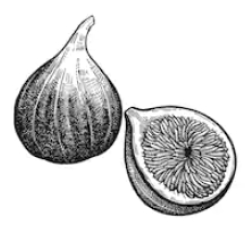
\includegraphics[width=1in,height=1.25in,clip,keepaspectratio]{fig1}}]{Michael Shell}
Use $\backslash${\tt{begin\{IEEEbiography\}}} and then for the 1st argument use $\backslash${\tt{includegraphics}} to declare and link the author photo.
Use the author name as the 3rd argument followed by the biography text.
\end{IEEEbiography}

\vspace{11pt}

\bf{If you will not include a photo:}\vspace{-33pt}
\begin{IEEEbiographynophoto}{John Doe}
Use $\backslash${\tt{begin\{IEEEbiographynophoto\}}} and the author name as the argument followed by the biography text.
\end{IEEEbiographynophoto}




\vfill

\end{document}


